\documentclass{article}
\usepackage{amsmath, amssymb}
\usepackage[english]{babel}
\usepackage{fullpage}
\usepackage{graphicx}
\usepackage[hidelinks]{hyperref}
\usepackage[round,authoryear]{natbib}
\bibliographystyle{plainnat}
\usepackage{microtype}

\author{Dieuwke Hupkes}
\title{Experiments}
\date{}

\begin{document}

\maketitle

% \section{Intro}

\section{Datasets}

I define the following set of languages:

\begin{table}[!ht]
\begin{tabular}{lccl}
    \textbf{Name} & \textit{Numeric leaves} & \textit{Tree depth} & \textit{Example}\\
    \hline
    $L_2$ & 2 & 1 & ($x_1$ \textit{op} $x_1$)\\
    $L_3$ & 3 & 2 & (($x_1$ \textit{op} $x_2$) \textit{op} $x_3$)\\
    $L_4$ & 4 & 3 & (($x_1$ \textit{op} $x_2$) \textit{op} ($x_3$ \textit{op} $x_4$))\\
    \dots& & &\\
\end{tabular}
\end{table}

\noindent Where $x_i\in\{-19,19\}$, and \textit{op} $\in\{+,-\}$. The meaning $y$ of e sentences is the result of the arithmetic expression expressed by the languag. We restrict the languages to include only expressions such that $y\in\{-60,60\}$.\\

\noindent We define the following (structurally non-ambiguous) subsets of the languages defined above:

\begin{table}[ht!]
\begin{tabular}{lll}
    \textbf{Name} & \textit{Restriction} & \textit{Example} \\
    \hline
    $L_i+$ & \textit{op} $==+$ & $(.(.(x_1 + x_2) + \dots x_i)$ \\
    $L_i-$ & \textit{op} $==-$ & $(.(.(x_1 - x_2) - \dots x_i)$ \\
    $L_i$rb & only right branching trees & $(.(.(x_1$ \textit{op} $x_2)$ \textit{op} $x_3)$ \textit{op} $\ldots x_i)$ \\
    $L_i$lb & only left branching trees & $(x_1$ \textit{op} $(x_2$ \textit{op} ($\ldots$ \textit{op} $(x_{i-1}$ \textit{op} $x_i).).)$ \\
\end{tabular}
\end{table}

The datasets that the networks will be trained and tested on are (subsets of) unions of the languages described above.

\section{Architectures}

I use four different architectures (explanation?):

\begin{figure}[!ht]
\setlength{\tabcolsep}{18pt}
\begin{tabular}{|cccc|}
    \hline
    \textbf{A1} & \textbf{A2} & \textbf{A3} & \textbf{A4}\\
    & & &\\
    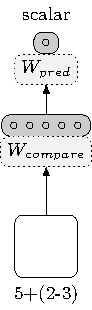
\includegraphics[scale=0.9]{A1} &
    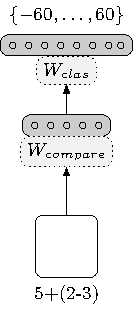
\includegraphics[scale=0.9]{A2} &
    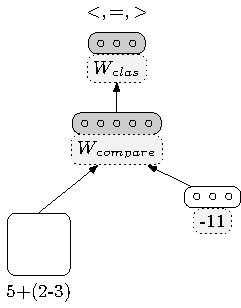
\includegraphics[scale=0.9]{A3} &
    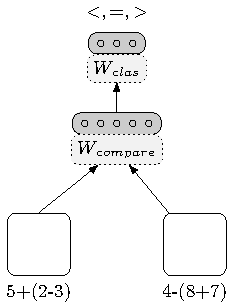
\includegraphics[scale=0.9]{A4}\\
\hline
\end{tabular}
\end{figure}


\section{Experiments}

I will start by running a sequence of experiments to determine if the networks can learn to compose the meaning of sentences from the structurally non ambiguous languages $L_2$, $L_3+$, $L_3-$, $L_3lb$ and $L_3rb$. Depending on the results I will move on to more complicated languages
In principle, I would like to do all (possible) combinations that can be made by combining elements from the following table,\footnote{Of course excluding non-sensical combinations, such as Gray encoding in two dimennions} starting with architectures A1 and A2 and then expanding to A3 and A4.

\begin{table}[!ht]
\begin{tabular}{|c|c|c|c|c|c|}
    \hline
    \textbf{Network} & \textbf{Language} & \textbf{Architecture} & \textbf{Dimensionality} & \textbf{Initialisation} & \textbf{Embeddings}\\
    \hline
    SRN & $L_2$   & A1    & 10    & Random    & fixed\\
    GRU & $L_3+$  & A2    & 6     & Gray      & trained\\
    LSTM & $L_3-$  & A3    & 2     & one-hot? &\\
    & $L_3rb$ & A4    & & &\\
    & $L_3lb$ &    & & &\\
    \hline
\end{tabular}
\end{table}

\section{More concrete plan}

Wat moet ik doen?
\begin{itemize}
    \item Generate datasets (or think of how to do that on the fly)
    \item Implement architectures
    \item Train networks and plot results
\end{itemize}

\end{document}
